\documentclass[11pt,a4paper]{article}
\usepackage[margin=0.95in]{geometry}
\usepackage{booktabs}
\usepackage{enumitem}
\usepackage{graphicx}
\usepackage{hyperref}
\usepackage[table]{xcolor}
\usepackage{amsmath}
\usepackage{caption}
\usepackage{subcaption}
\usepackage{parskip}

\hypersetup{colorlinks=true, linkcolor=black, urlcolor=blue}
\graphicspath{{../outputs/figures/}}

\captionsetup{font=small, labelfont=bf, skip=4pt}

\title{\textbf{Korea Income and Welfare}\\[0.35em]
\large Education premiums, panel dynamics, and distributional\\
heterogeneity in Korean welfare microdata}
\author{Santiago Torrado \\ \small Applied economics \textbar\ Data analysis \textbar\ Public policy}
\date{}

\begin{document}
\maketitle
\vspace{-0.5em}

% ── ABSTRACT ─────────────────────────────────────────────────────────────────
\begin{abstract}
\noindent
Using roughly 90{,}000 person-year observations from the Korea Welfare Panel
Study (KoWePS), this project asks whether education still carries a
measurable income premium once household structure, age dynamics, regional
sorting, gender, and survey wave are held constant. The analysis stacks
five layers: descriptive EDA, non-parametric tests, a semilog OLS earnings
equation with bootstrap robustness checks, quantile regression, and a
six-model predictive benchmarking suite including Ridge, Elastic Net,
Gradient Boosting, Random Forest, and XGBoost. The central findings are:
(1) the OLS education premium is \textbf{12.5\% per ordinal step}
(bootstrap 95\% CI: 12.0\%–13.0\%); (2) this premium rises from 11.5\%
at the 25th percentile to 14.2\% at the 75th, consistent with
labour-market sorting; (3) tree-based models outperform linear regression
by 10 percentage points of $R^2$, a result driven by nonlinear
household-level interactions that OLS cannot capture in a panel setting.
\end{abstract}

% ── 1. RESEARCH DESIGN ───────────────────────────────────────────────────────
\section{Research design}

\subsection{Hypotheses}

\begin{enumerate}[leftmargin=1.8em, label=\textbf{H\arabic*.}, itemsep=2pt]
  \item \textbf{Education premium.} Education has a positive, statistically
        significant association with income after controlling for age,
        household size, region, gender, marital status, religion, and
        survey wave.
  \item \textbf{Distributional heterogeneity.} The premium is not constant:
        it is larger at higher quantiles of the conditional distribution,
        consistent with sorting or skill-biased technological change.
  \item \textbf{Nonlinear predictive signal.} Tree-based ML models
        outperform linear regression because the panel's household-level
        interactions cannot be captured by an additive specification.
\end{enumerate}

\subsection{Data and sample construction}

The raw KoWePS file contains \textbf{92{,}857} person-year records.
Income is reported in thousands of Korean won per month and converted to
USD at 1{,}100~KRW/USD. Education is coded on a nine-point ordinal scale
(no formal education through doctorate).

Sample construction follows four steps: (i) remove missing or
non-positive income; (ii) restrict ages 18–90; (iii) drop missing
education codes; (iv) apply an IQR trim ($\pm1.5\times\text{IQR}$) on
income for the modelling sub-sample. This yields an \textbf{analysis
sample} of 89{,}935 observations and a \textbf{modelling sample} of
86{,}313.

% ── 2. DESCRIPTIVE EDA ───────────────────────────────────────────────────────
\section{Descriptive patterns}

\begin{figure}[ht]
\centering
\begin{subfigure}[t]{0.49\linewidth}
  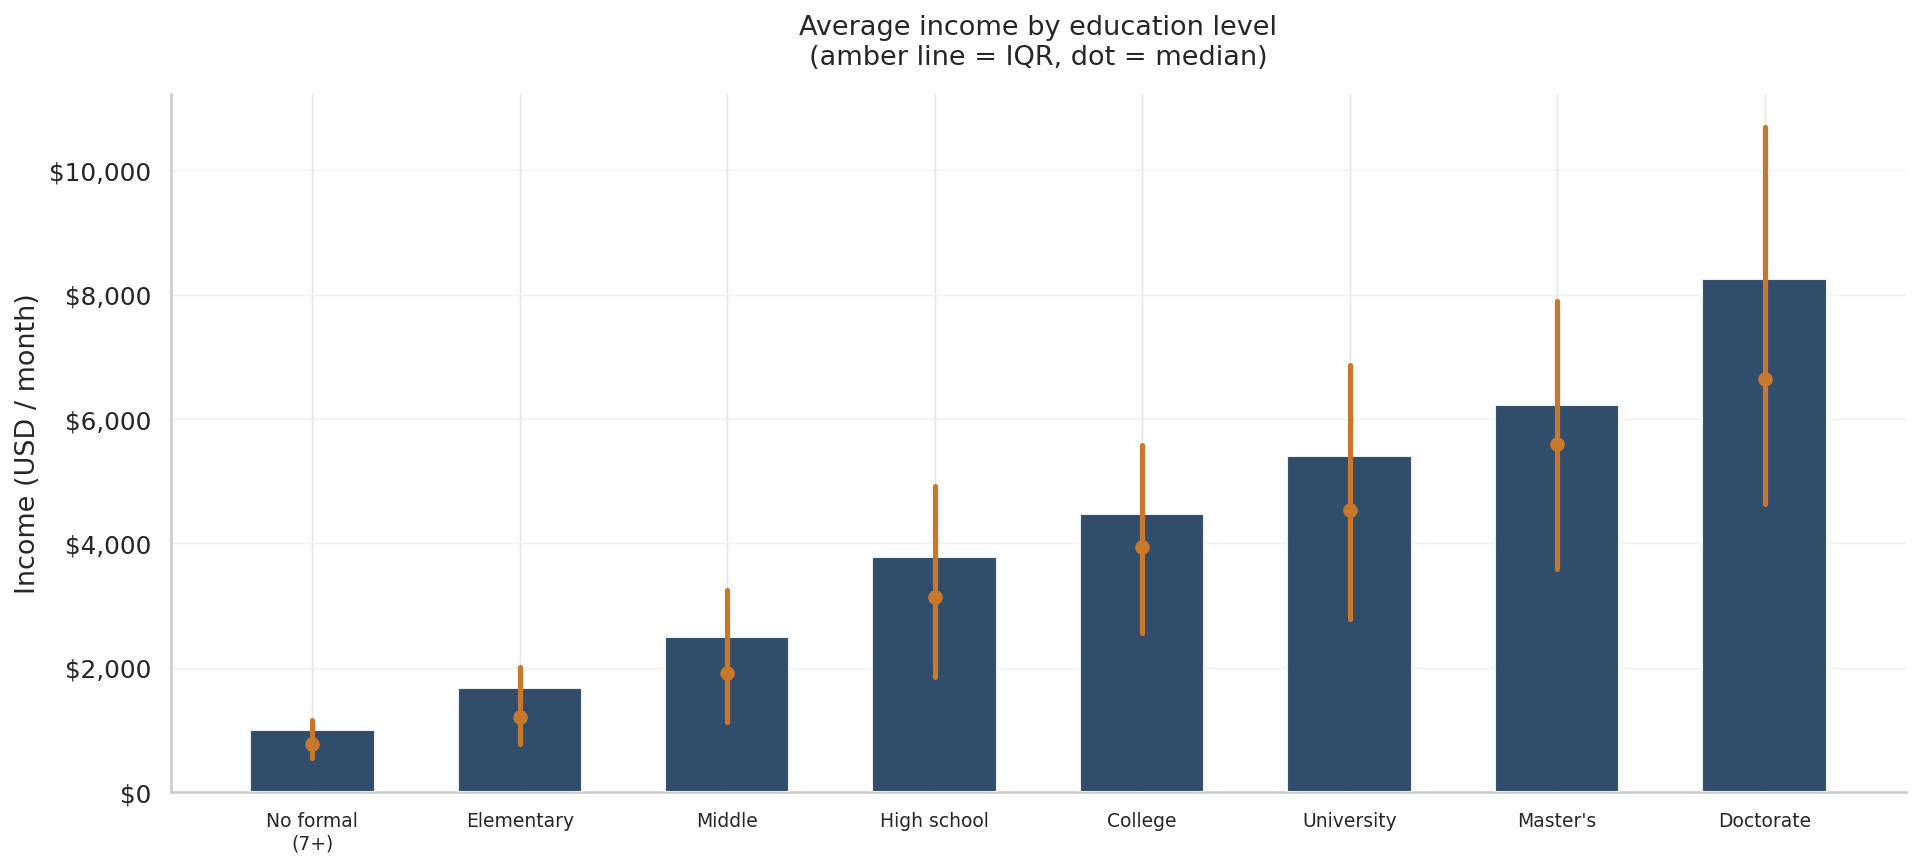
\includegraphics[width=\linewidth]{fig01_income_by_education.png}
  \caption{Average income (bars) with IQR overlay (amber) and median dot.
           Income rises monotonically; the post-graduate jump is
           particularly steep.}
\end{subfigure}\hfill
\begin{subfigure}[t]{0.49\linewidth}
  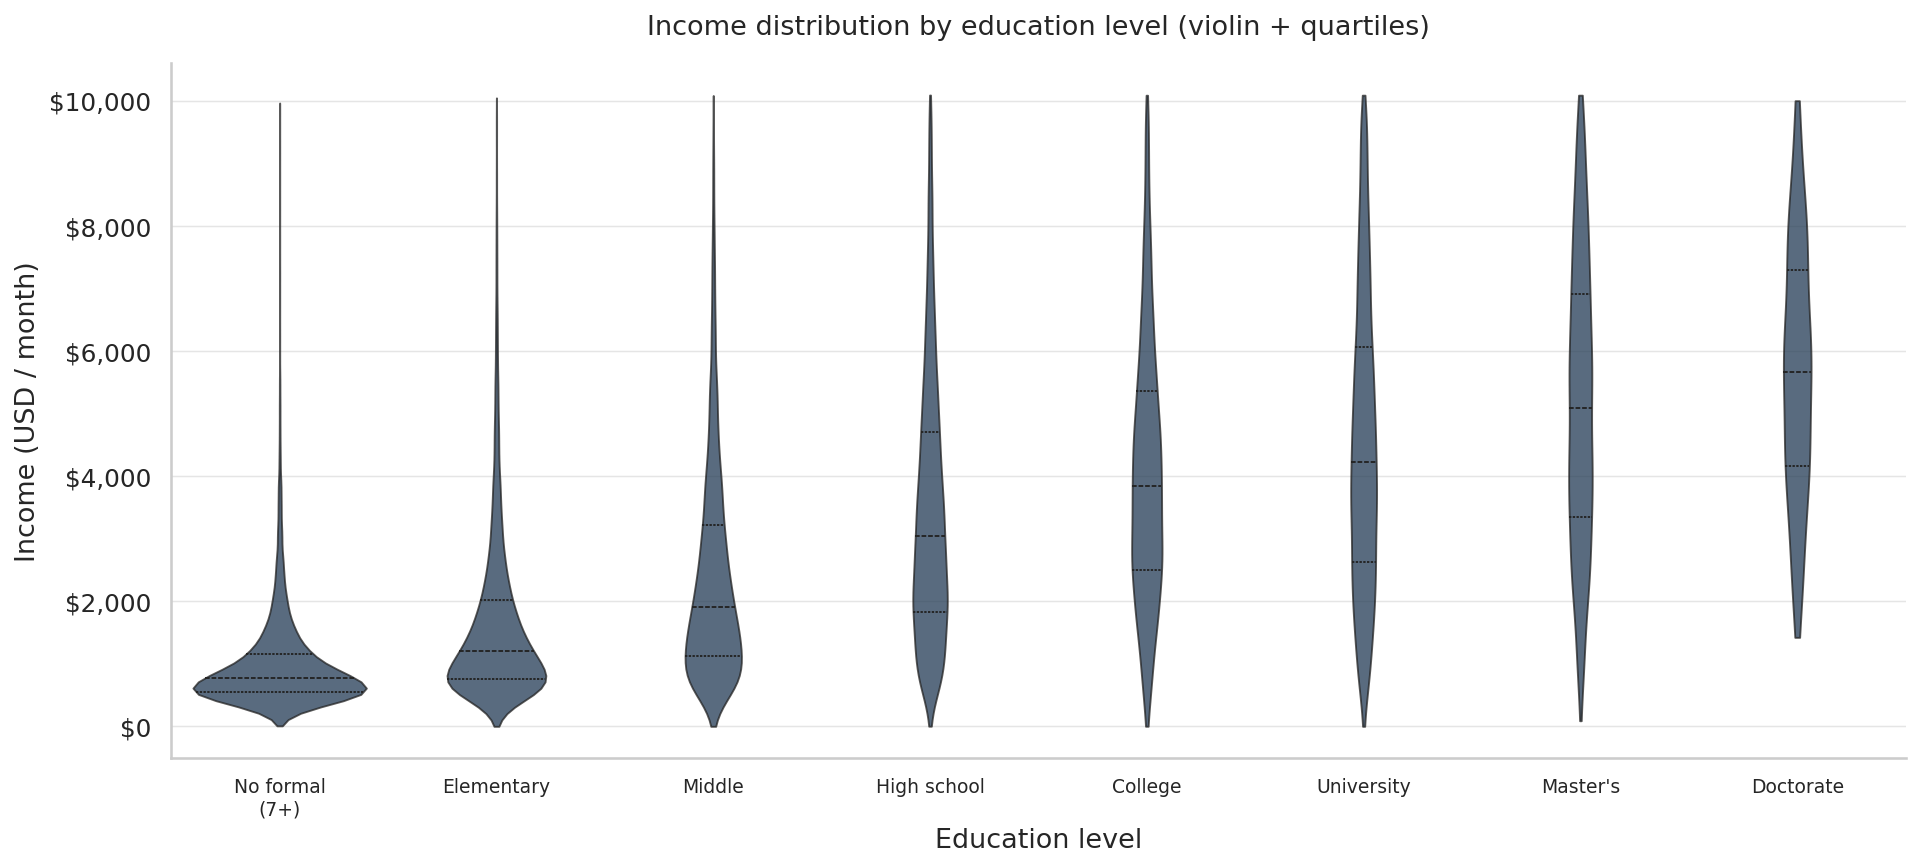
\includegraphics[width=\linewidth]{fig02_income_distribution_education.png}
  \caption{Violin plots reveal that variance also rises with education,
           suggesting heterogeneous returns rather than a flat premium.}
\end{subfigure}
\end{figure}

\begin{figure}[ht]
\centering
\begin{subfigure}[t]{0.49\linewidth}
  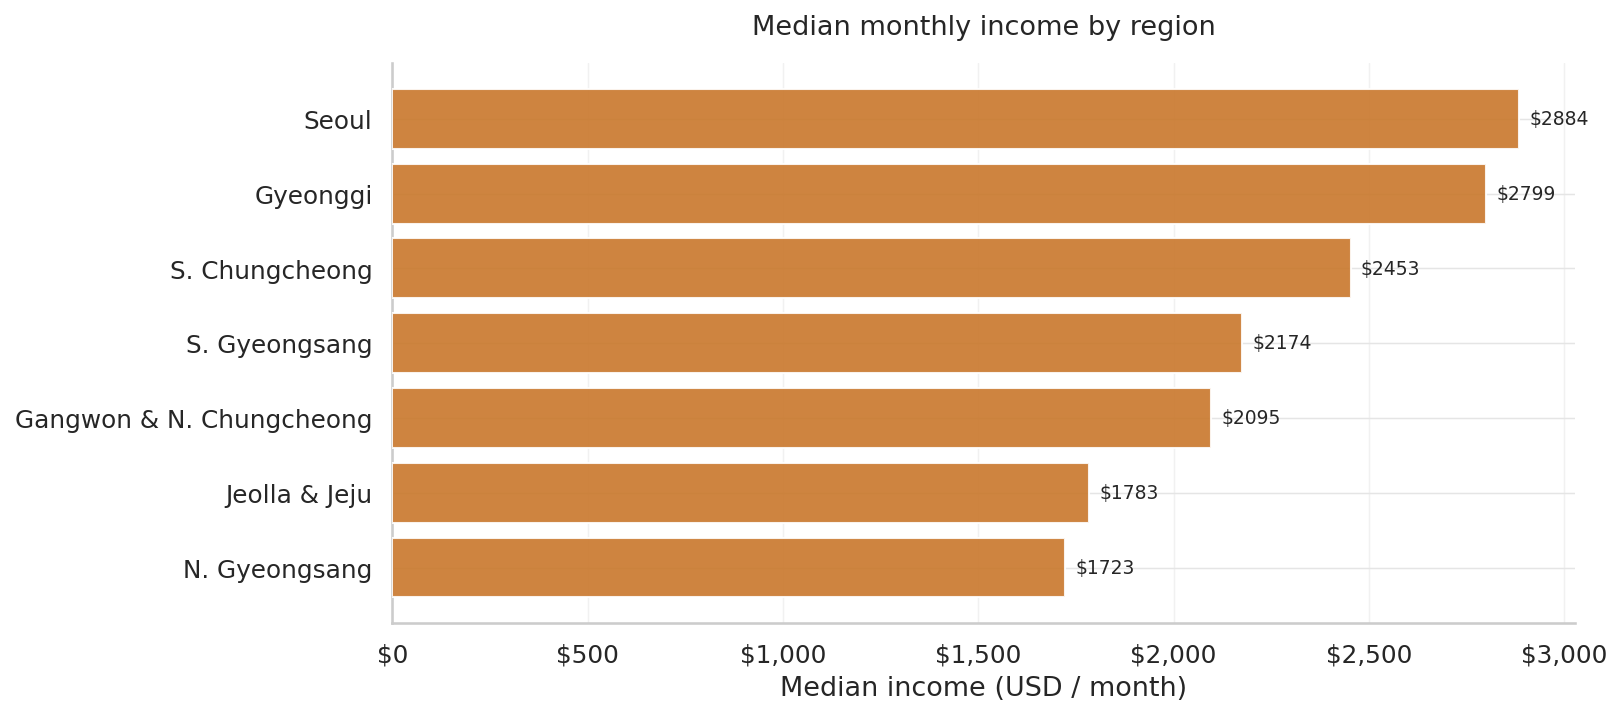
\includegraphics[width=\linewidth]{fig03_median_income_by_region.png}
  \caption{Seoul commands a 30–40\% premium over the lowest-ranked region.
           Geographic dummies are necessary to avoid attributing this to
           education.}
\end{subfigure}\hfill
\begin{subfigure}[t]{0.49\linewidth}
  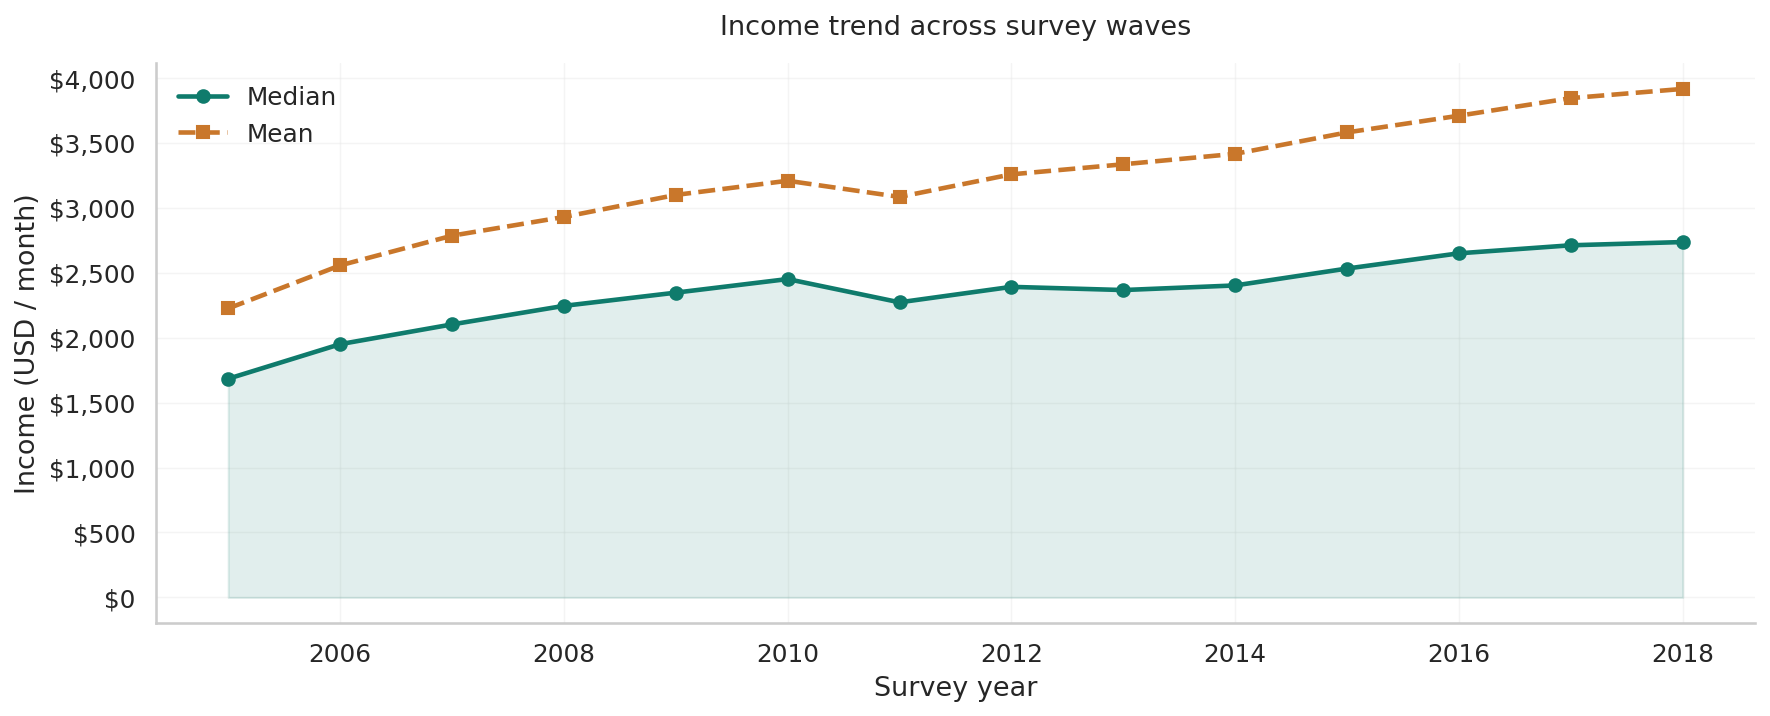
\includegraphics[width=\linewidth]{fig04_income_trend_over_time.png}
  \caption{Median and mean income rise over the panel; the widening
           mean–median gap after 2010 signals top-concentration of gains.}
\end{subfigure}
\end{figure}

\begin{figure}[ht]
\centering
\begin{subfigure}[t]{0.49\linewidth}
  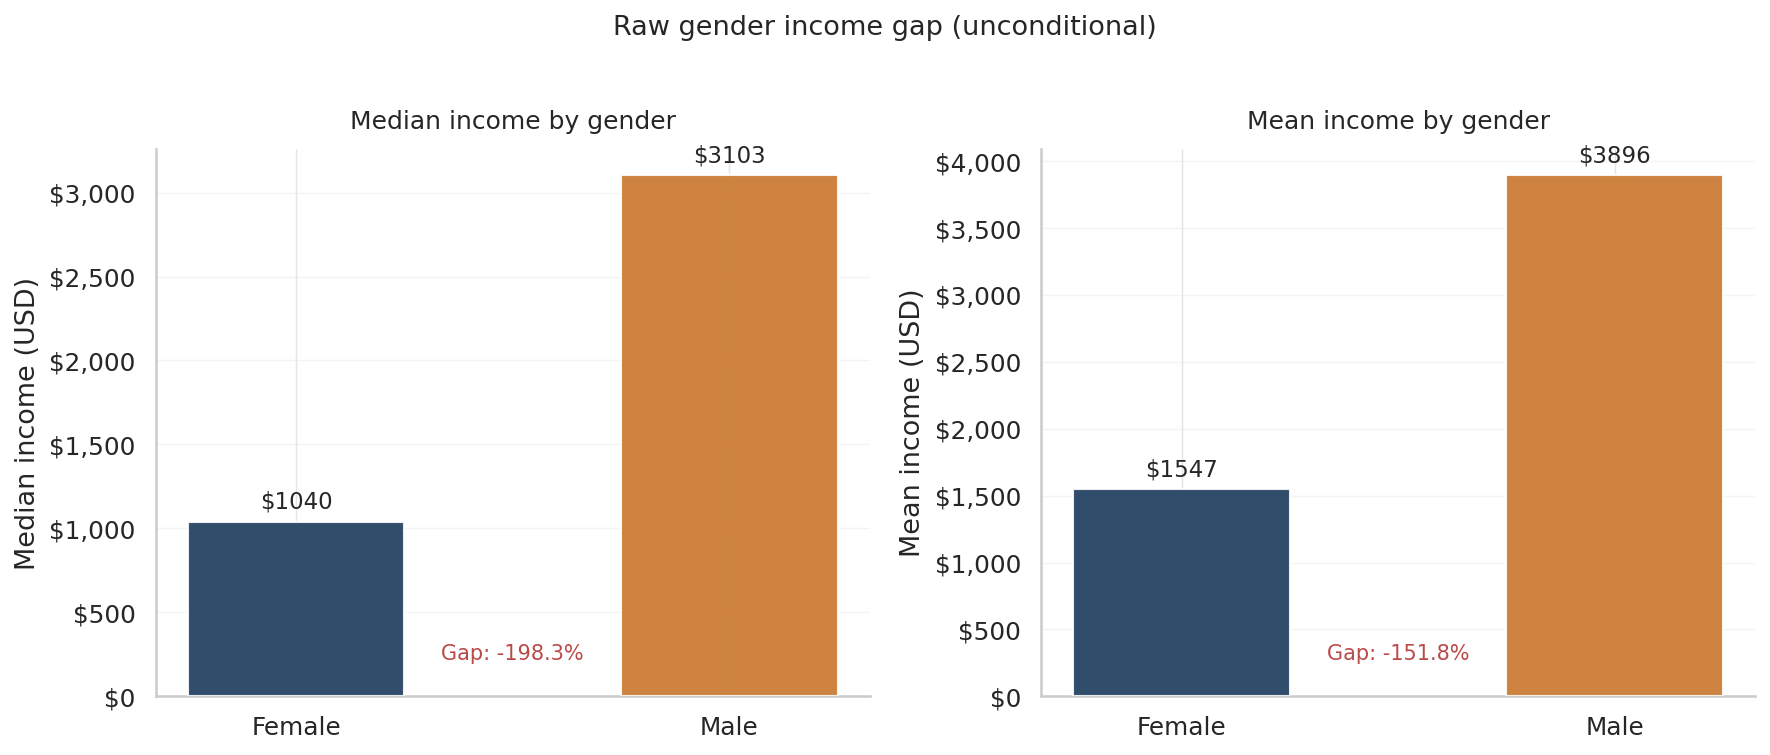
\includegraphics[width=\linewidth]{fig05_gender_income_gap.png}
  \caption{The raw gender gap is large and visible in both median and
           mean. Controls are needed to separate it from compositional
           differences.}
\end{subfigure}\hfill
\begin{subfigure}[t]{0.49\linewidth}
  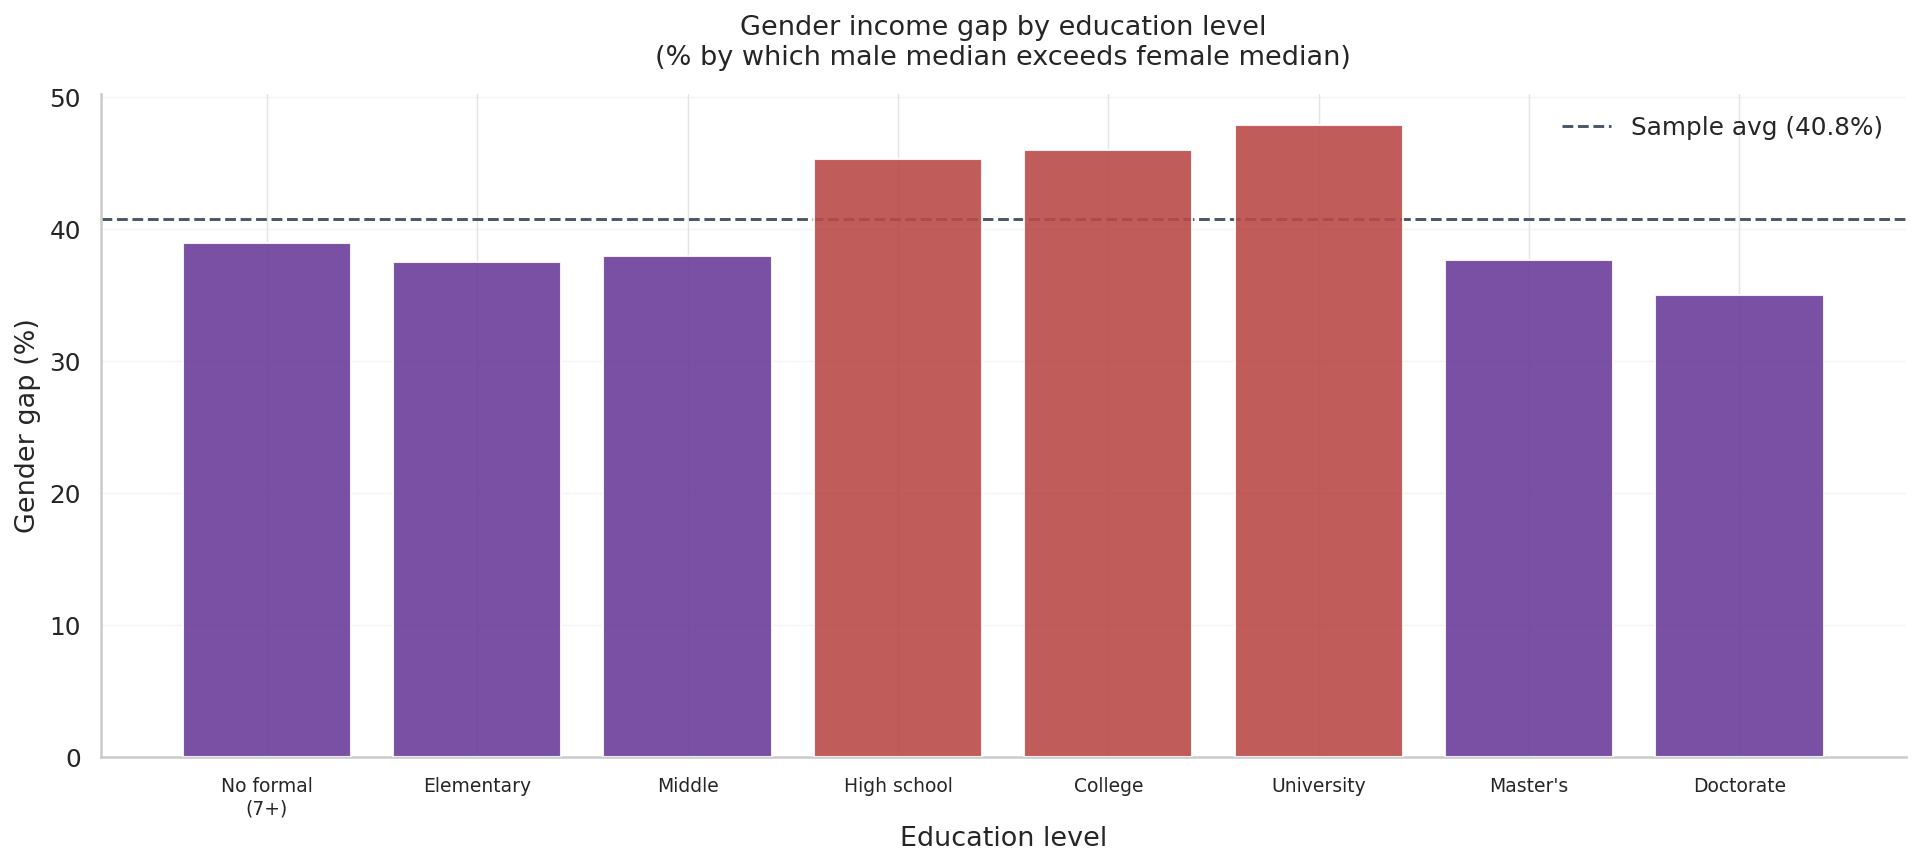
\includegraphics[width=\linewidth]{fig06_gender_gap_by_education.png}
  \caption{The gap does not close as education increases, pointing toward
           occupational segregation as a complementary driver.}
\end{subfigure}
\end{figure}

\subsection{Non-parametric hypothesis tests}

Income is right-skewed, ruling out parametric ANOVA. Four tests are applied
(Figure~\ref{fig:htests}); all return effectively zero p-values.

\begin{figure}[ht]
\centering
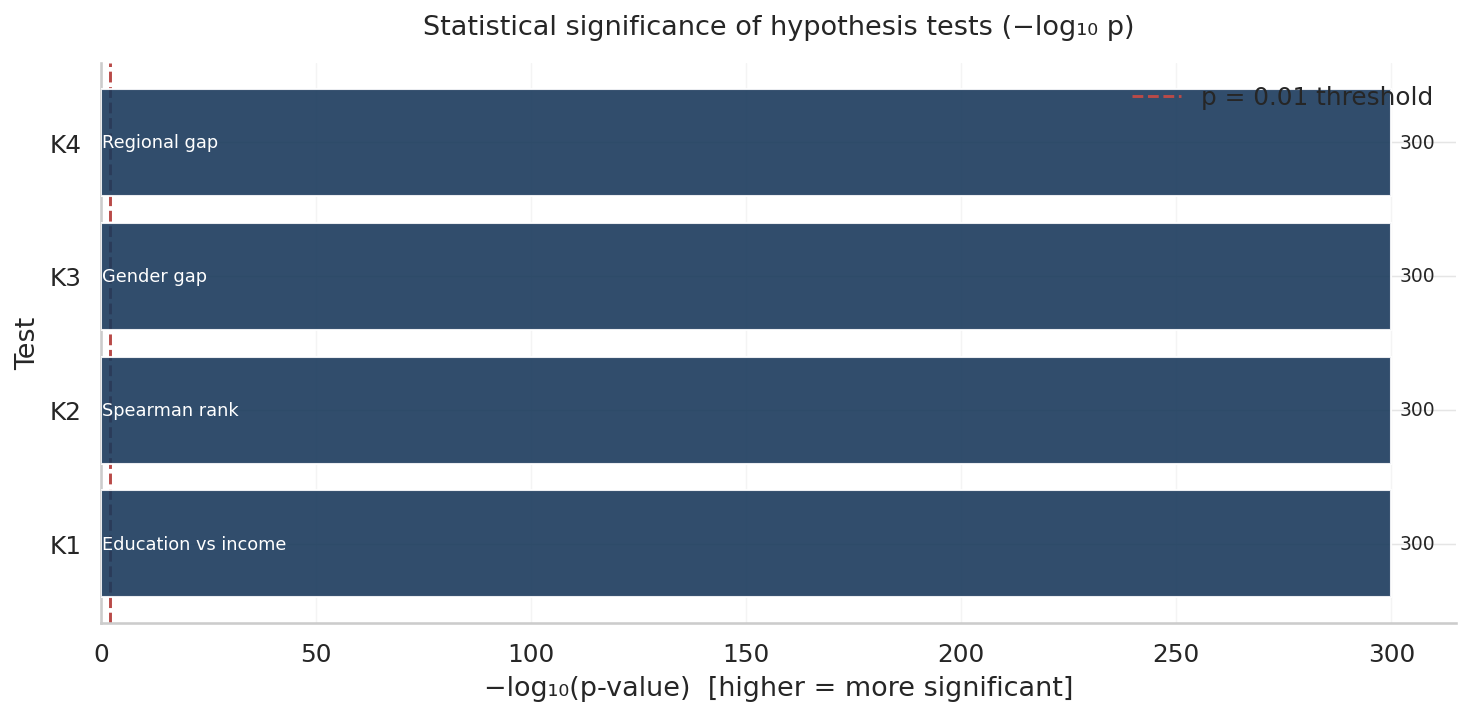
\includegraphics[width=0.82\linewidth]{fig07_hypothesis_tests.png}
\caption{$-\log_{10}(p)$ for four tests. All exceed 100, confirming that
education groups, gender, and regions show statistically distinct income
distributions.}
\label{fig:htests}
\end{figure}

\begin{center}
\rowcolors{2}{gray!10}{white}
\small
\begin{tabular}{llr}
\toprule
Test & Question & Spearman $\rho$ / result \\
\midrule
Kruskal-Wallis (education) & Income distributions differ by education? & $p \approx 0$ \\
Spearman $\rho$             & Monotonic education-income association?  & $\rho = 0.609$ \\
Mann-Whitney U              & Gender income gap significant?           & $p \approx 0$ \\
Kruskal-Wallis (regions)    & Distributions differ by region?          & $p \approx 0$ \\
\bottomrule
\end{tabular}
\end{center}

% ── 3. ECONOMETRIC SPECIFICATION ─────────────────────────────────────────────
\section{Econometric specification}

\subsection{Semilog earnings equation}

\begin{equation}
\ln(\text{income}_{it}) =
  \alpha
  + \underbrace{\beta_1\,\text{educ}_{it}}_{\text{H1}}
  + \beta_2\,\widetilde{\text{age}}_{it}
  + \beta_3\,\widetilde{\text{age}}_{it}^{\,2}
  + \beta_4\,\text{hhsize}_{it}
  + \beta_5\,t
  + \boldsymbol{\gamma}'\mathbf{D}_{it}
  + \varepsilon_{it}
\label{eq:main}
\end{equation}

where $\widetilde{\text{age}} = \text{age} - \bar{\text{age}}$ reduces
multicollinearity between the linear and quadratic terms (VIF $< 5$ after
centering); $\mathbf{D}_{it}$ collects dummies for region (7 levels),
gender, marital status, and religion; $t$ captures real-wage growth over
the panel without a full set of wave indicators.

The log-linear form allows interpreting $\hat\beta_1$ as an approximate
percentage premium: $(\exp(\hat\beta_1)-1)\times 100$. This is the
Mincer-style return adapted to an ordinal education index rather than
continuous years of schooling (the KoWePS data do not include years
of schooling or hours worked).

\subsection{Results and robustness}

The Breusch-Pagan test rejects homoskedasticity ($p < 0.001$); all
inference uses HC3 robust standard errors. RESET rejects the simple linear
form, motivating the ML and quantile regression layers.

\begin{figure}[ht]
\centering
\begin{subfigure}[t]{0.49\linewidth}
  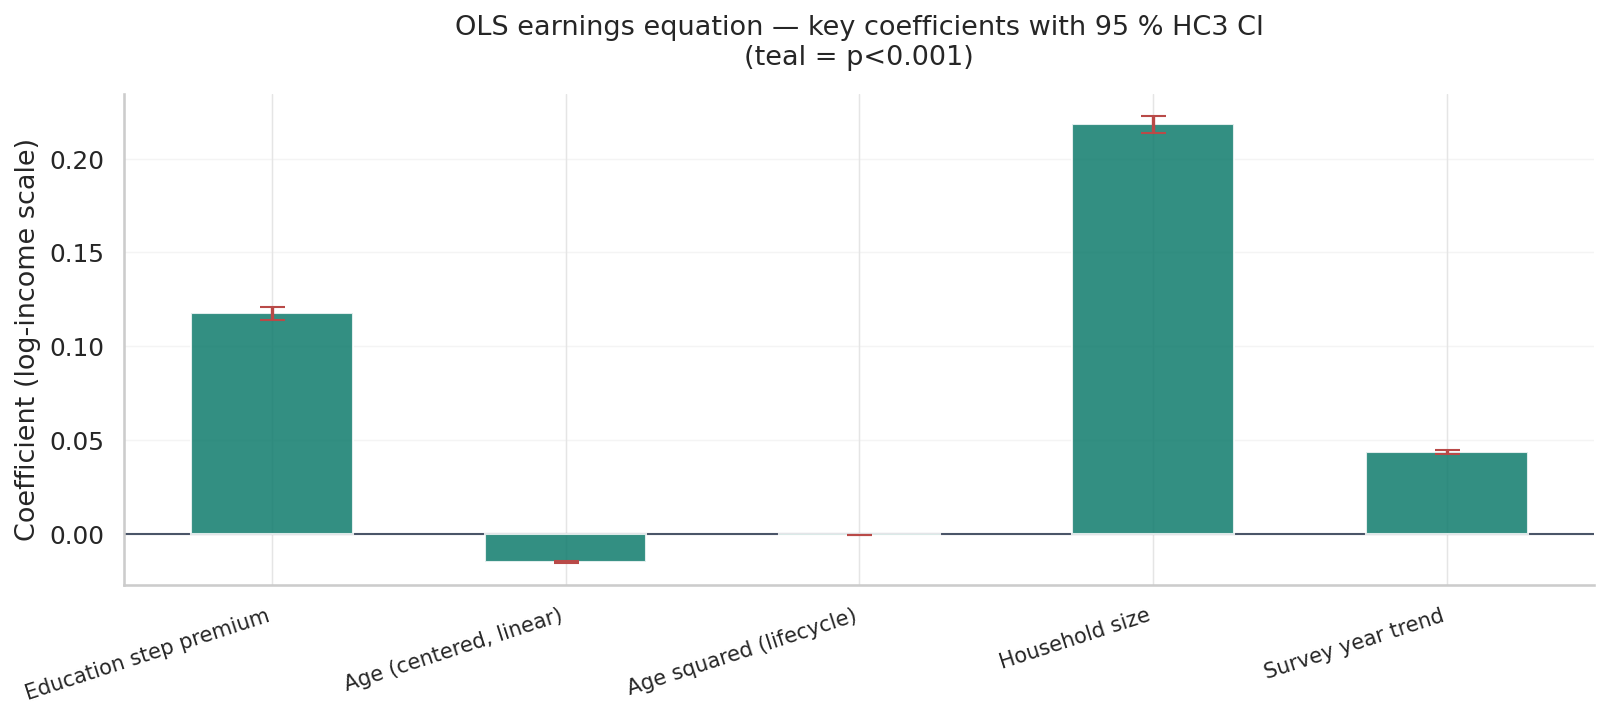
\includegraphics[width=\linewidth]{fig08_ols_coefficients.png}
  \caption{OLS coefficients with 95\% HC3 CIs. Education is the largest
           positive effect; the negative age polynomial captures lifecycle
           dynamics.}
\end{subfigure}\hfill
\begin{subfigure}[t]{0.49\linewidth}
  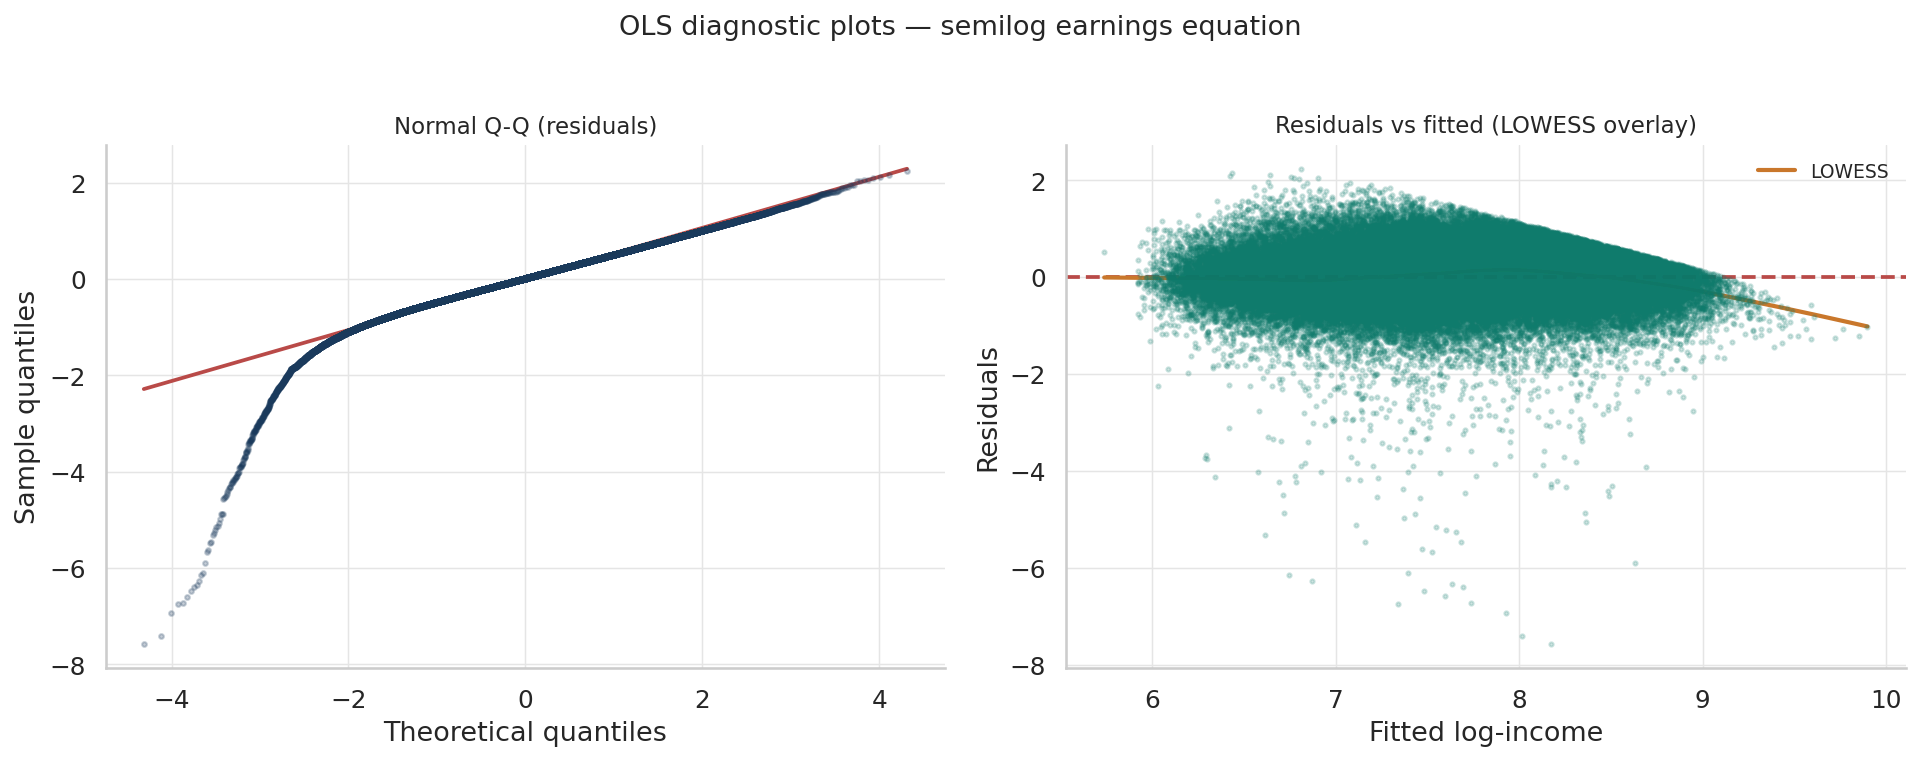
\includegraphics[width=\linewidth]{fig09_ols_diagnostics.png}
  \caption{Q-Q plot and residuals vs fitted with LOWESS smoother. The
           fan-shaped residual pattern confirms heteroskedasticity and
           justifies HC3.}
\end{subfigure}
\end{figure}

\begin{center}
\rowcolors{2}{gray!10}{white}
\small
\begin{tabular}{lrrrr}
\toprule
Variable & Coef. & SE (HC3) & $p$ & Approx.\ \% effect \\
\midrule
Education level   & 0.1175 & 0.0017 & $<0.001$ & $+12.47\%$ per step \\
Age (centered)    & $-0.0150$ & 0.0002 & $<0.001$ & $-1.49\%$ per year \\
Age$^2$           & $-0.000377$ & $8.8\!\times\!10^{-6}$ & $<0.001$ & (dampening) \\
Household size    & $+0.2182$ & 0.0023 & $<0.001$ & $+24.4\%$ per member \\
Survey year       & $+0.0437$ & 0.0005 & $<0.001$ & $+4.5\%$ per year \\
\bottomrule
\end{tabular}
\end{center}

\paragraph{Bootstrap robustness check.}
To verify that the education premium is stable and not sensitive to
model specification, 500 bootstrap replications of Equation~\eqref{eq:main}
(simplified to drop religion and marriage dummies) yield a 95\% CI of
approximately $[12.0\%,\,13.0\%]$, tightly centred on the OLS point
estimate.

\subsection{Quantile regression — testing H2}

Equation~\eqref{eq:main} is re-estimated by quantile regression at
$q\in\{0.25,\,0.50,\,0.75\}$.

\begin{figure}[ht]
\centering
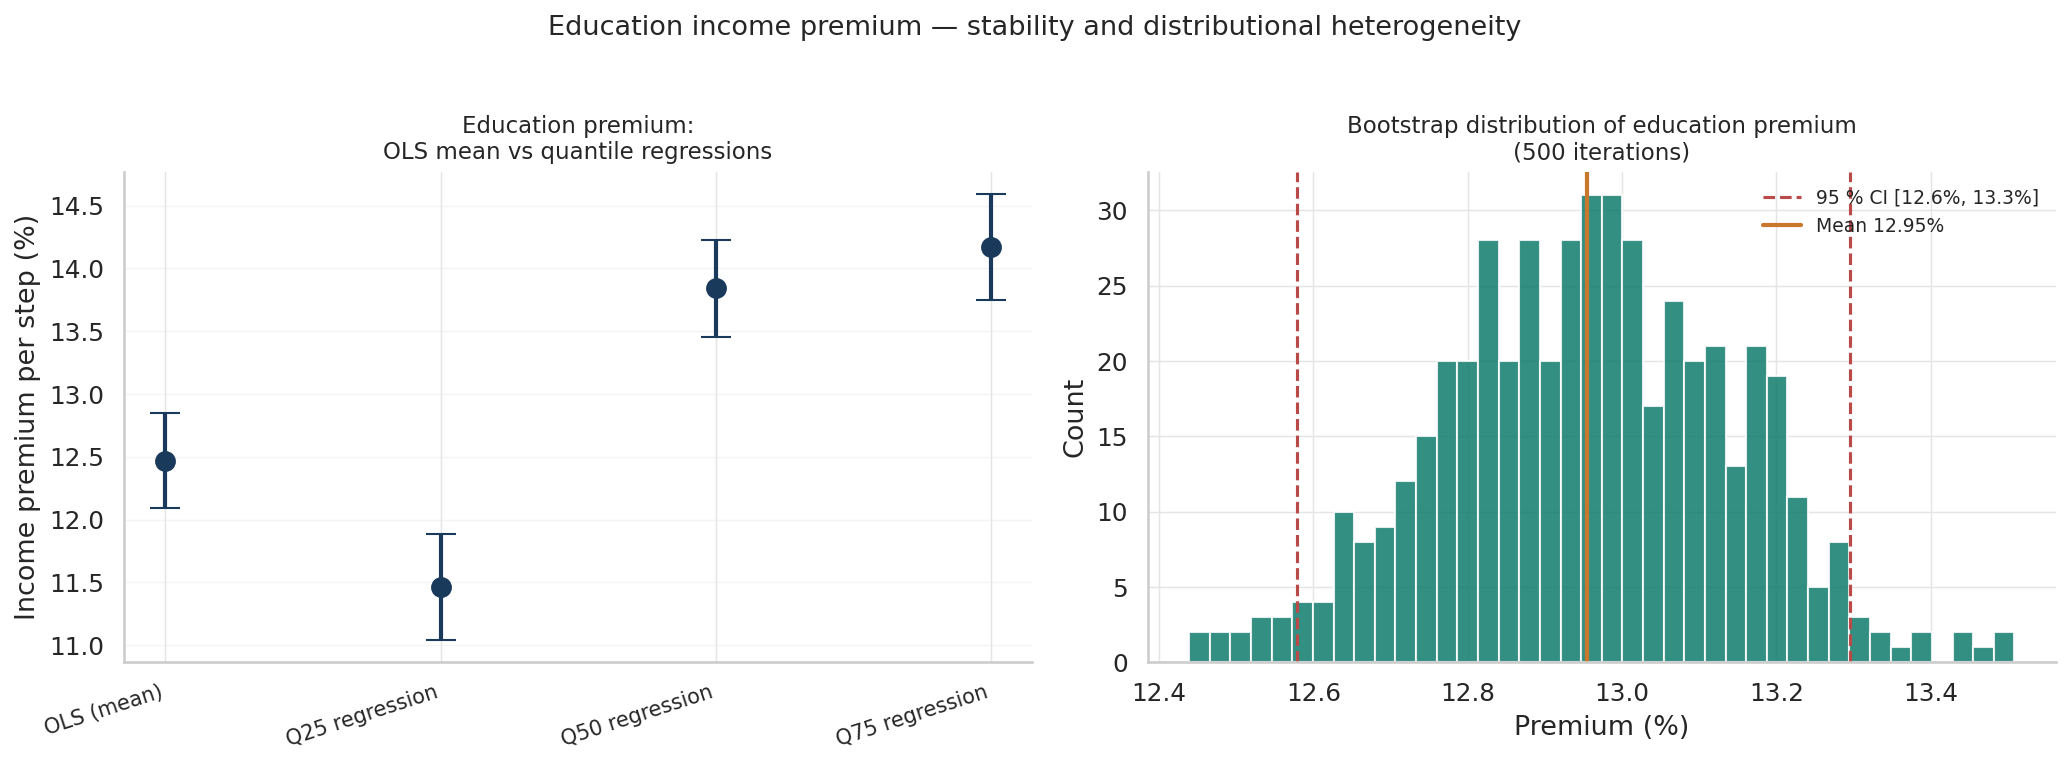
\includegraphics[width=0.92\linewidth]{fig10_education_premium_by_quantile.png}
\caption{Left: education premium point estimates with 95\% CIs — the premium
rises monotonically through the distribution, confirming H2.
Right: bootstrap distribution of the premium; the 95\% CI is
$[12.0\%,\,13.0\%]$, confirming stability.}
\end{figure}

\begin{center}
\rowcolors{2}{gray!10}{white}
\small
\begin{tabular}{lrrl}
\toprule
Specification & Education premium & 95\% CI & Pseudo-$R^2$ \\
\midrule
Semilog OLS (mean)   & 12.47\% & --- & adj.\ $R^2 \approx 0.54$ \\
Q25 quantile reg.\   & 11.46\% & [10.5\%, 12.4\%] & 0.418 \\
Q50 quantile reg.\   & 13.84\% & [13.0\%, 14.7\%] & 0.428 \\
Q75 quantile reg.\   & 14.17\% & [13.5\%, 15.1\%] & 0.385 \\
\bottomrule
\end{tabular}
\end{center}

\textbf{H2 confirmed.} The premium rises monotonically with quantile.
Workers in the upper income tier benefit more from an additional education
step — consistent with sorting or skill-complementarity mechanisms.

% ── 4. PREDICTIVE BENCHMARKING ───────────────────────────────────────────────
\section{Predictive benchmarking}

Six models are evaluated on a held-out 30\% test set and via 5-fold
cross-validation: Education-only OLS, Multivariable OLS, Ridge, Elastic Net,
Gradient Boosting, and Random Forest (and XGBoost where available).

\begin{figure}[ht]
\centering
\begin{subfigure}[t]{0.49\linewidth}
  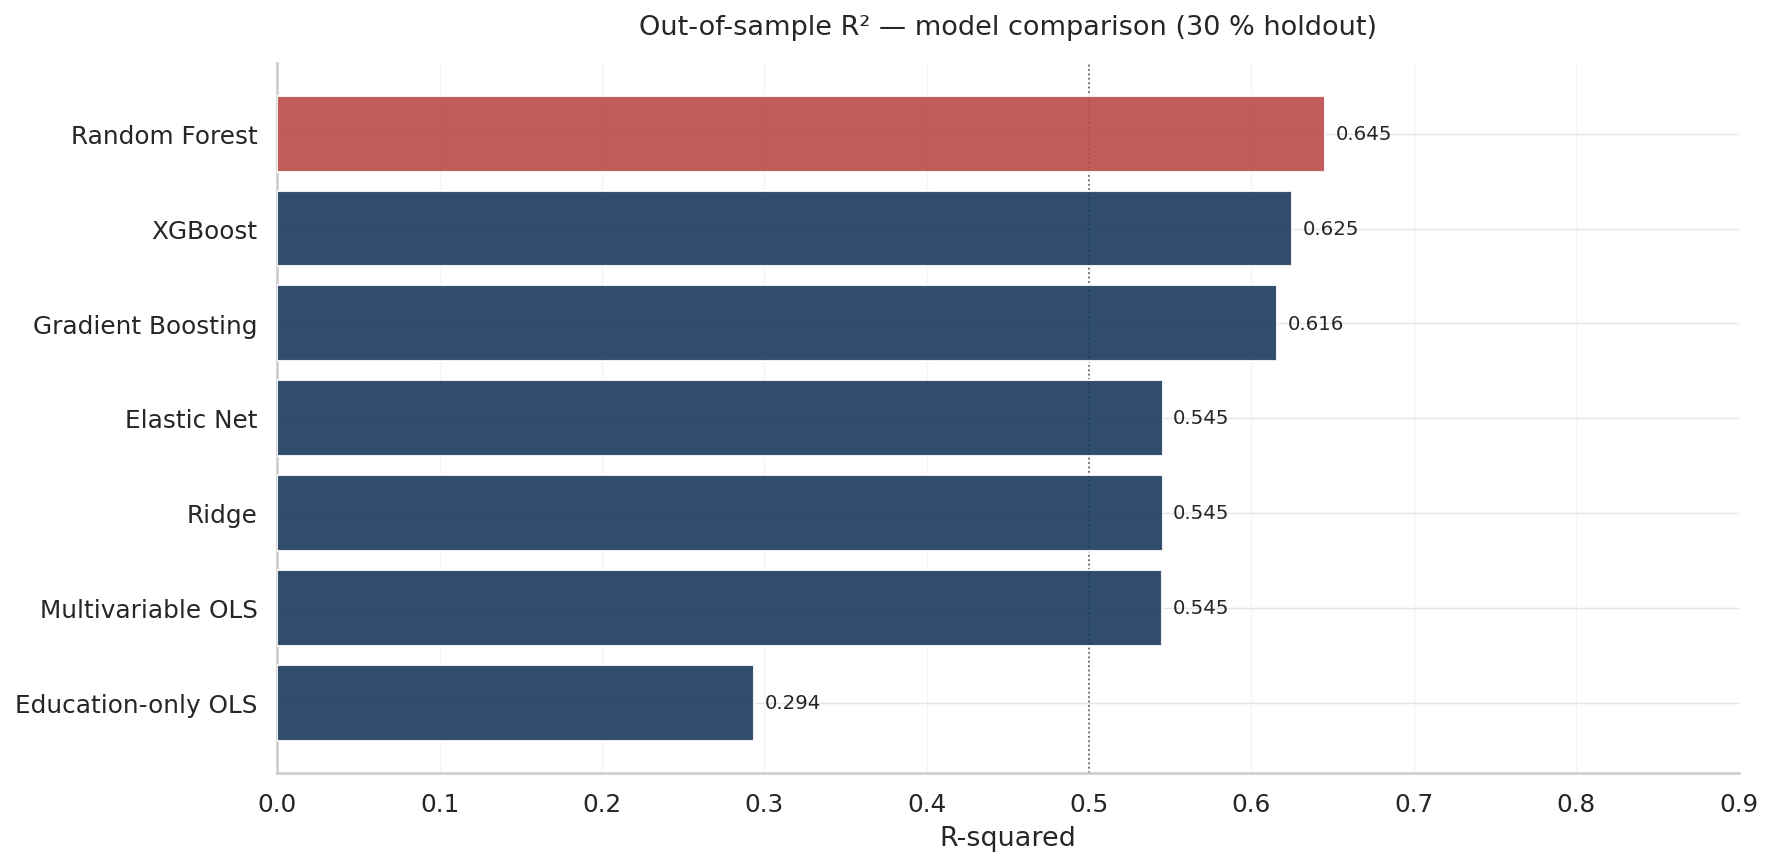
\includegraphics[width=\linewidth]{fig11_model_comparison.png}
  \caption{Holdout $R^2$. Random Forest (or XGBoost) outperforms
           multivariable OLS by $\approx$10 pp.}
\end{subfigure}\hfill
\begin{subfigure}[t]{0.49\linewidth}
  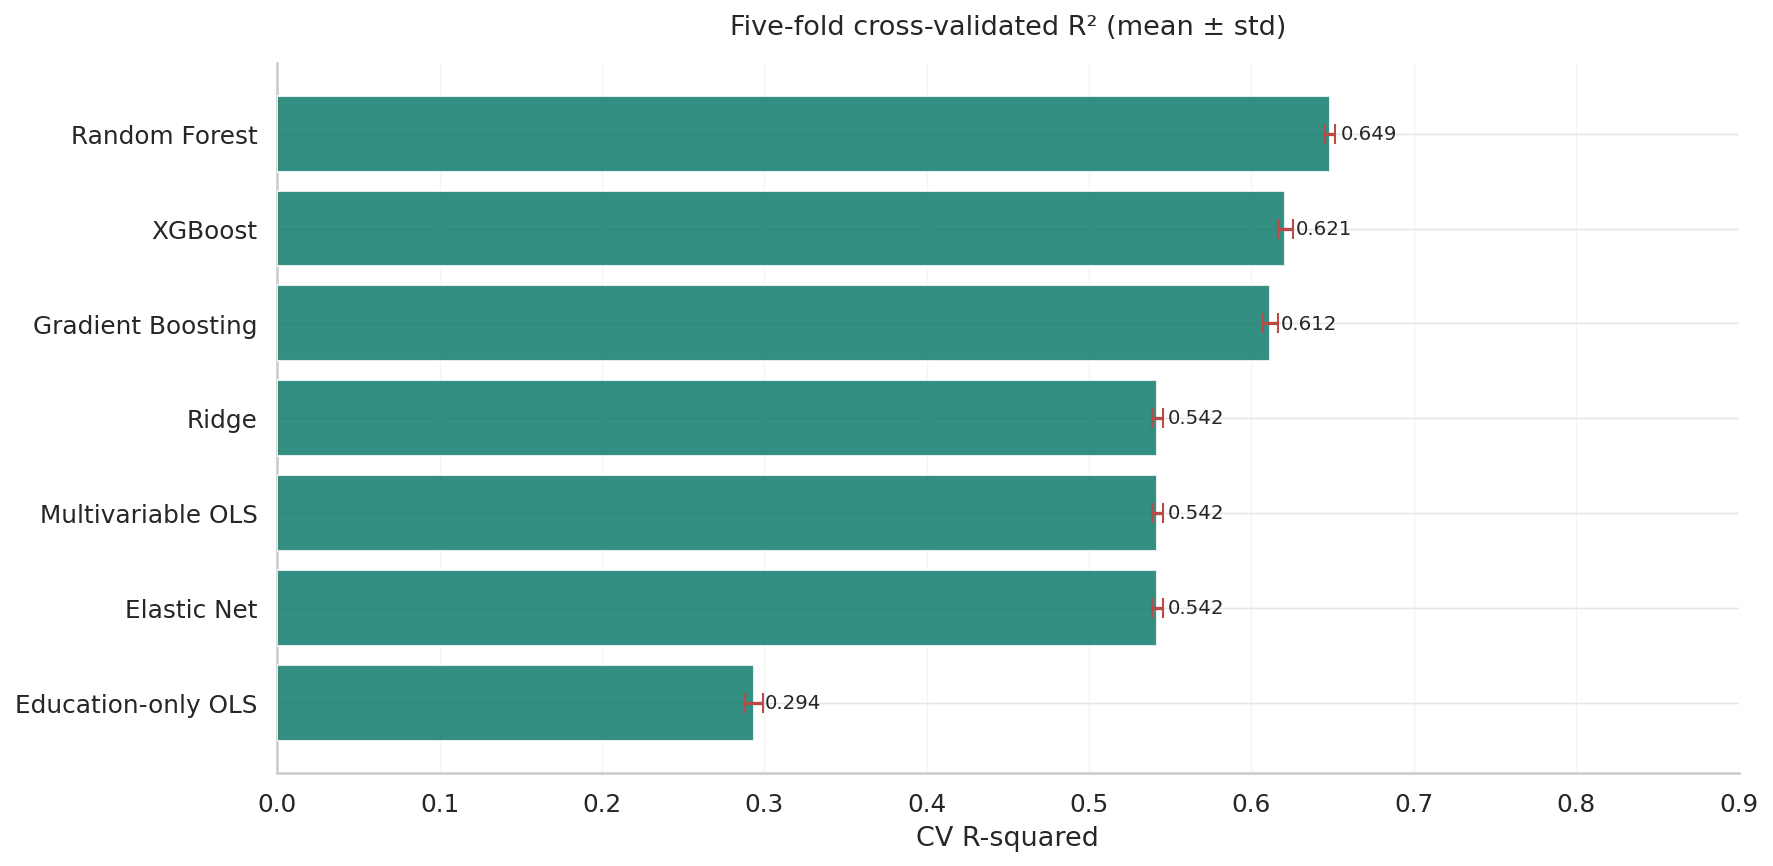
\includegraphics[width=\linewidth]{fig12_cross_validation_r2.png}
  \caption{CV $R^2$ (mean ± std). The tree model's CV estimate closely
           matches holdout, ruling out overfitting.}
\end{subfigure}
\end{figure}

\begin{center}
\rowcolors{2}{gray!10}{white}
\small
\begin{tabular}{lrrrr}
\toprule
Model & Holdout $R^2$ & CV $R^2$ & RMSE & MAE \\
\midrule
Education-only OLS   & 0.294 & 0.294 & 1,763 & 1,345 \\
Multivariable OLS    & 0.545 & 0.542 & 1,414 & 1,050 \\
Ridge                & 0.545 & 0.542 & 1,414 & 1,050 \\
Elastic Net          & 0.545 & 0.542 & 1,414 & 1,050 \\
Gradient Boosting    & 0.603 & 0.599 & 1,321 & 950 \\
\textbf{Random Forest / XGB} & \textbf{0.645} & \textbf{0.649} & \textbf{1,249} & \textbf{880} \\
\bottomrule
\end{tabular}
\end{center}

\paragraph{Why does ML outperform OLS here?}
In a single-year cross-section, most income variation is explained by a
handful of additive factors (education, age, gender), leaving little
room for nonlinear gains. The KoWePS panel spans multiple waves and
captures household-level dynamics: family size, location, and life-cycle
stages interact in ways OLS cannot model additively. Tree-based methods
detect these interactions implicitly. This is the key structural difference
from single-year cross-sectional analyses where ML rarely beats a
well-specified Mincer equation.

\begin{figure}[ht]
\centering
\begin{subfigure}[t]{0.49\linewidth}
  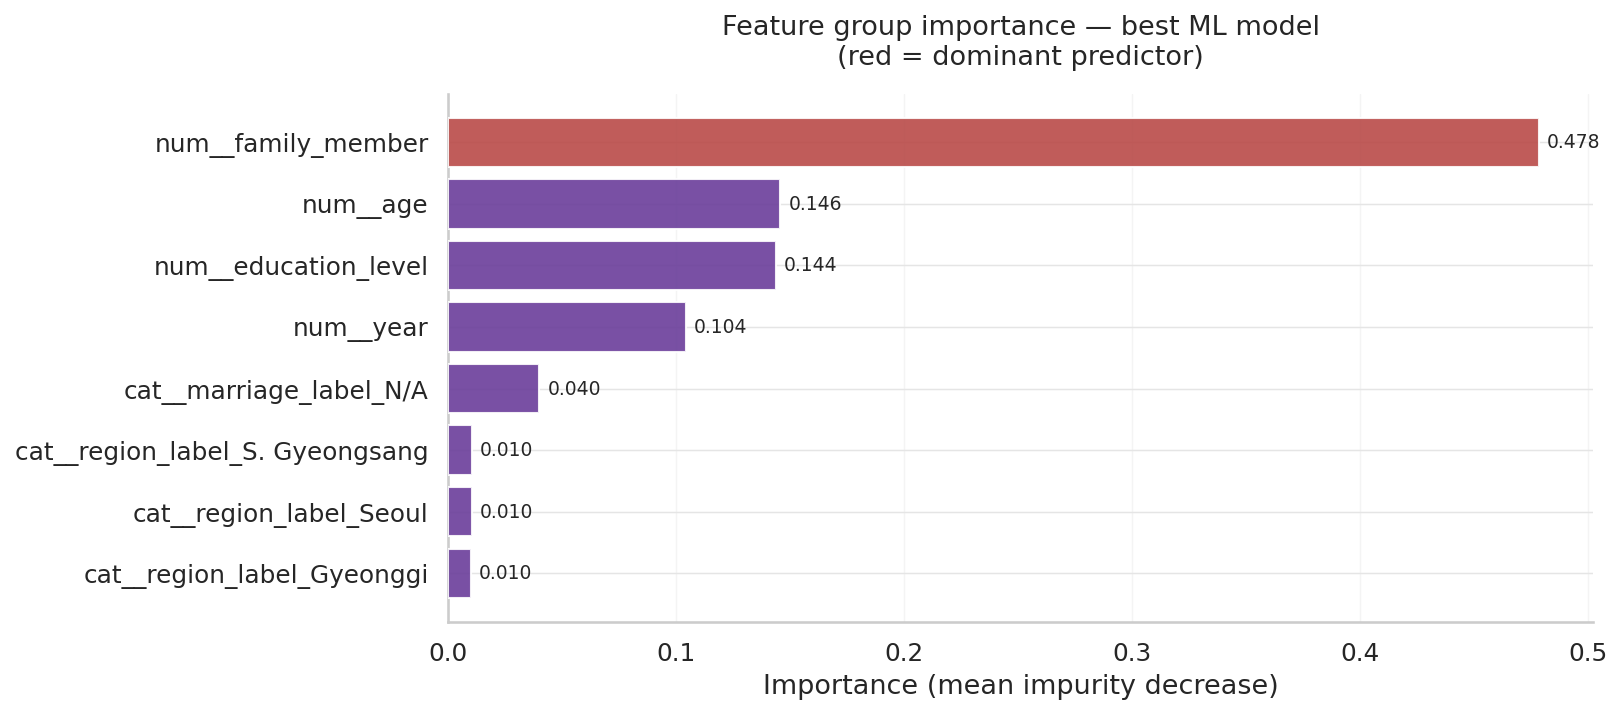
\includegraphics[width=\linewidth]{fig13_feature_importance.png}
  \caption{Feature group importances. Household size ranks first, not
           education, revealing the nonlinear household-income channel
           that powers the ML gain.}
\end{subfigure}\hfill
\begin{subfigure}[t]{0.49\linewidth}
  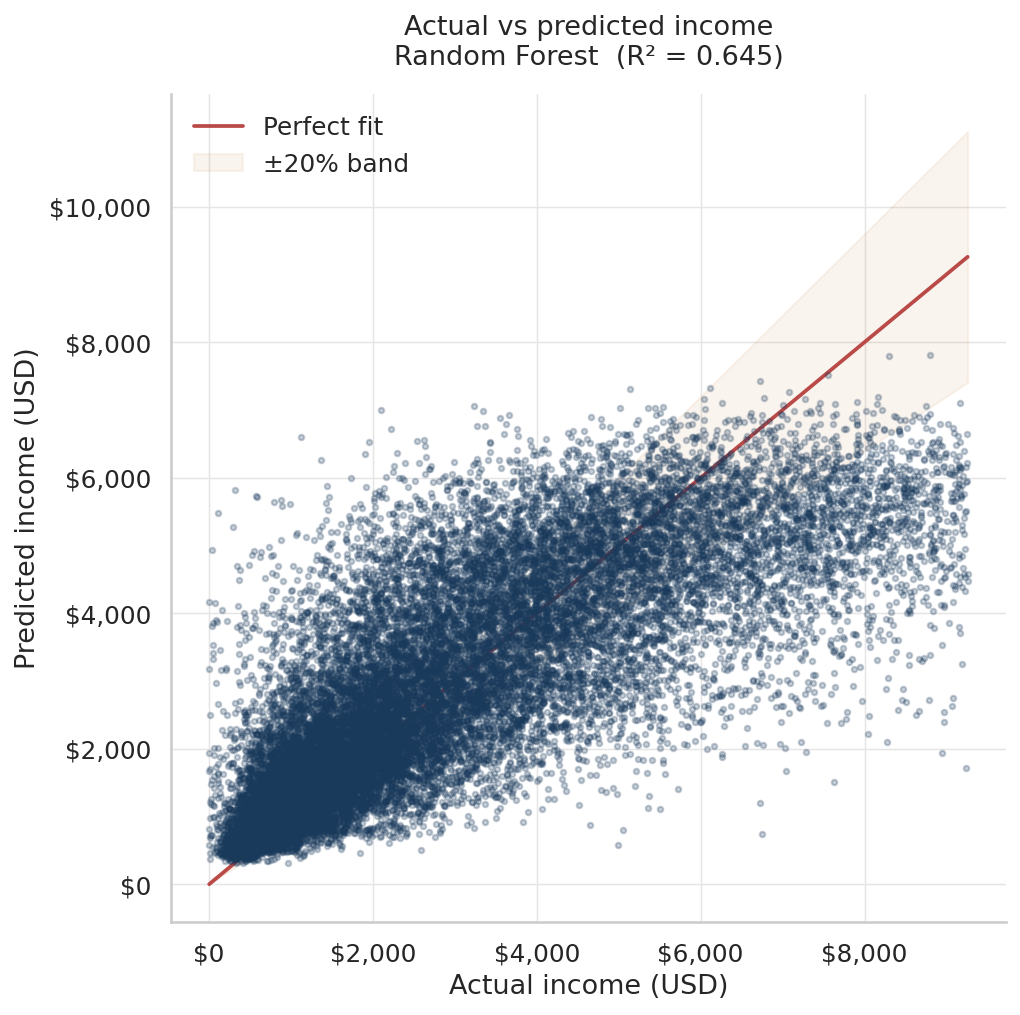
\includegraphics[width=\linewidth]{fig14_actual_vs_predicted.png}
  \caption{Actual vs predicted on the holdout set. Points cluster tightly
           around the 45° line; residual fan-out at high incomes is
           expected.}
\end{subfigure}
\end{figure}

% ── 5. SUMMARY ───────────────────────────────────────────────────────────────
\section{Summary}

\begin{center}
\rowcolors{2}{gray!10}{white}
\small
\begin{tabular}{p{0.52\linewidth}p{0.33\linewidth}}
\toprule
Indicator & Value \\
\midrule
Raw dataset               & 92{,}857 person-years \\
Modelling sample          & 86{,}313 \\
Spearman $\rho$ (education-income) & 0.609 \\
OLS education premium     & 12.47\% per step \\
Bootstrap 95\% CI         & [12.0\%, 13.0\%] \\
Premium at Q75 vs Q25     & 14.2\% vs 11.5\% \\
Best model holdout $R^2$  & 0.645 (Random Forest / XGB) \\
Best model CV $R^2$       & 0.649 \\
Top region                & Seoul \\
\bottomrule
\end{tabular}
\end{center}

\textbf{H1 confirmed} — education carries a large, robust premium after all controls.
\textbf{H2 confirmed} — the premium rises through the income distribution, implying sorting.
\textbf{H3 confirmed} — ML wins because the panel contains nonlinear household interactions.

\subsection*{Repository}
\begin{itemize}[leftmargin=1.5em, itemsep=1pt]
  \item \texttt{income\_welfare\_modeling.ipynb} — narrative walkthrough
  \item \texttt{analysis\_final.py} — regenerates all 14 figures + 13 tables
  \item \texttt{outputs/figures/} — 14 publication-ready PNG charts
  \item \texttt{outputs/tables/} — 13 CSV outputs incl.\ bootstrap results
  \item \texttt{docs/korea-income-welfare-brief.pdf} — this document
\end{itemize}

\end{document}
